% Put labels, etc., on figures using PSTricks.
% Use dvips -E <file>.dvi -o <file>.eps to create encapsulated PostScript.
%
\documentclass[12pt]{article}
\usepackage{graphicx}
\usepackage{pstricks}
\pagestyle{empty}

\begin{document}
\rput(5,-5){
\rput(.1,-.1){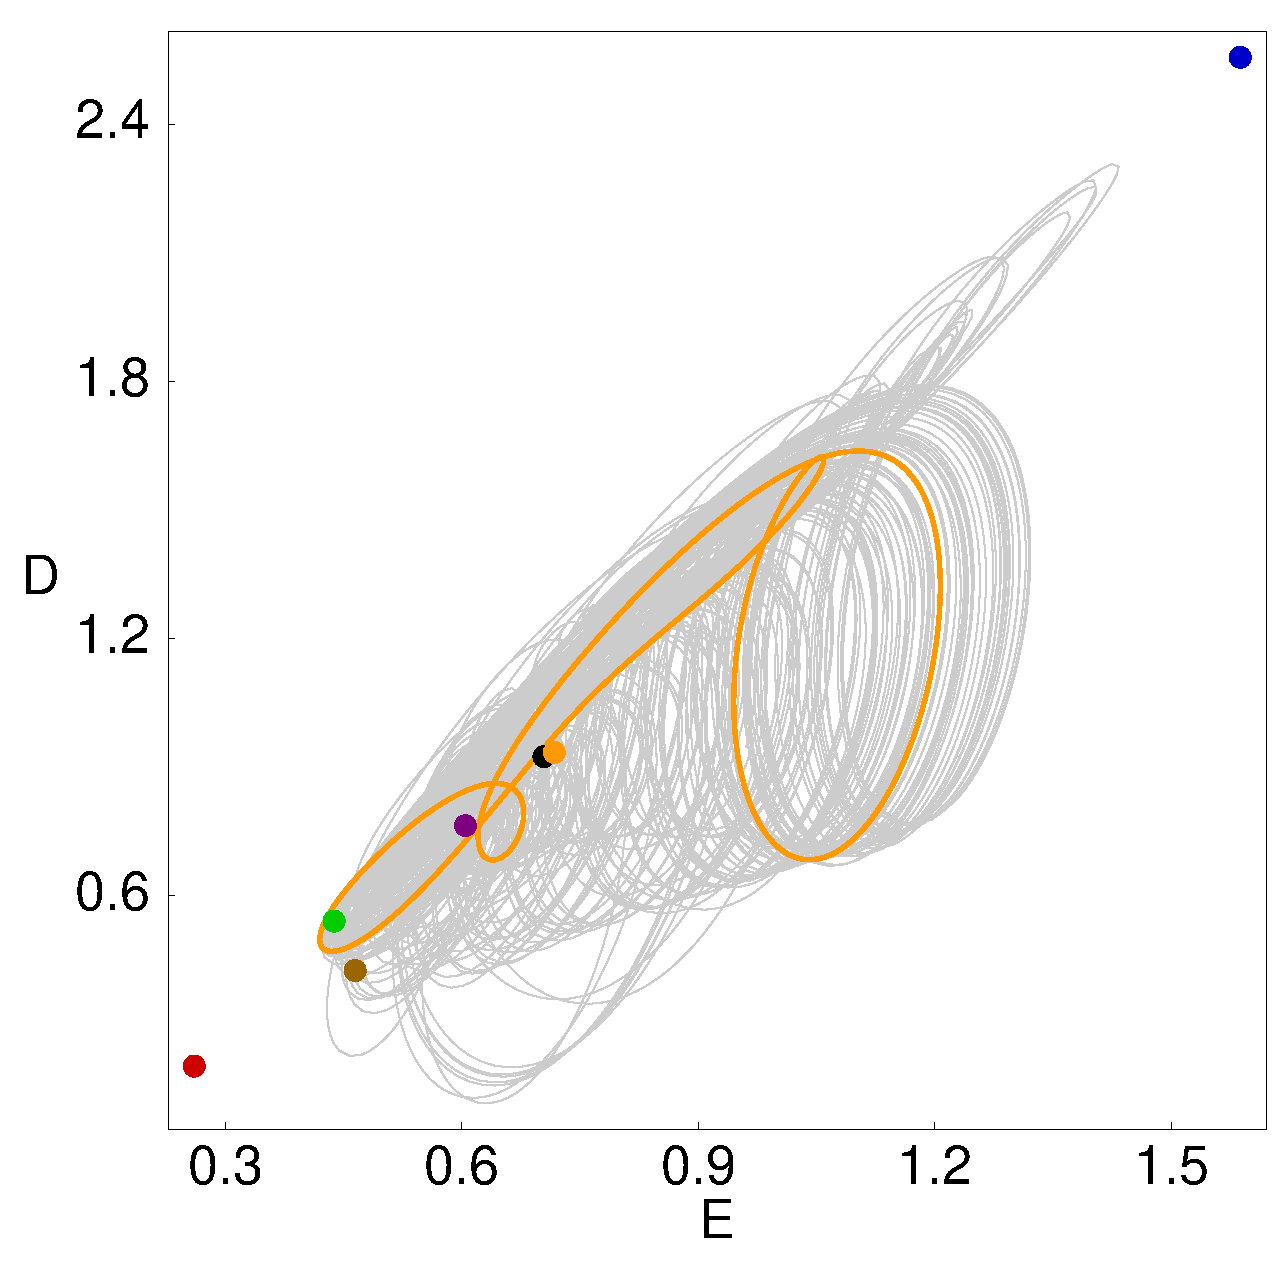
\includegraphics{../../rpo_ks/figs/EDequiva.eps}}

\huge

\psframe*[linecolor=white](-6.5,6)(-5.5,7)
\psframe*[linecolor=white](6,-6.5)(7.2,-5.5)

\rput(8.9,8.9){E$_3$} \rput(-6.8,-6.8){E$_1$}

\psline[linewidth=2pt]{->}(-6.5,-3.9)(-5.15,-4.7)\rput(-7,-3.8){E$_2$}
\psline[linewidth=2pt]{->}(0.2,-6.4)(-4.7,-5.55)\rput(1.5,-6.5){TW$_{\pm1}$}
\psline[linewidth=2pt]{->}(-5.3,-2)(-3.1,-3.1)\rput(-6,-1.5){TW$_{\pm2}$}
\psline[linewidth=2pt]{->}(0,6.5)(3.4,4)\rput(0,7){``Turbulence''}
\psline[linewidth=2pt]{->}(4,-5.5)(3.1,-3.5)\rput(7,-5.5){$T\simeq 33\,, l\simeq 11$}
\psline[linewidth=2pt]{->}(-2,2.5)(-1.6,-1.8)\rput(-3,4){$T\simeq 33\,, l\simeq 11$,}\rput(-3,3){Time Average}
\psline[linewidth=2pt]{->}(-5,0)(-1.85,-1.95)\rput(-5,1.5){``Turbulence'',}\rput(-5.,0.5){Time Average}


% Use grid command below to place objects at specified coordinates.
%\psgrid[subgriddiv=1,griddots=10](-8,-8)(10,10)
}
\end{document}
